\section{Magnetoterapia e ettromagnetoterapia}

L'applicazione di campi magnetici ed elettromagnetici è utilizzata nelle
valutazioni in ambito diagnostico ma è anche utilizzata come forma di
energia e di stimolazione che può dare effetti terapeutici.

\emph{La magnetoterapia è una terapia basata sull'utilizzo di
\textbf{solenoidi} di diverse dimensioni in grado di formare un campo
magnetico intorno al segmento corporeo presso i quali li si pone.}

\emph{Un campo elettrico variabile può produrre un campo magnetico
variabile.} Di conseguenza, tramite un campo elettrico, possiamo avere
un'onda elettromagnetica. Le onde elettromagnetiche si propagano con la
stessa frequenza della corrente che le ha prodotte. Noi siamo bombardati
da onde elettromagnetiche dovunque, perché siamo sempre a contatto con
correnti elettriche di diversa frequenza.

\section{Interazione tra campo magnetico e sistemi biologici}

\emph{In realtà non è ancora ben conosciuta la modalità tramite cui i
campi magnetici interagiscono con}

\emph{l'organismo. Il campo magnetico esercita azione sulla componente
ionica dell'organismo, quindi influenza processi di migrazione degli
ioni e delle molecole cariche elettricamente.}

\emph{A \textbf{livello cellulare} le maggiori attività influenzate
sono:}
\begin{itemize}

\item \emph{pompa K/Na}

\item \emph{flusso di ioni Ca}

\item \emph{inoltre potrebbe influenzare la permeabilità di membrana.}
\end{itemize}

Il campo magnetico che si crea per induzione di un campo elettrico ha
degli effetti biologici importanti.

\textbf{Effetti primari:} attività meccanica ed elettrica.

\textbf{Effetti secondari:} reazioni chimiche, fisiche, di risonanza,
termici.

\subsection{Effetti magnetomeccanici }

Sono effetti diretti legati all'interazione del campo magnetico con:

\begin{itemize}
\item[1.]
  dei materiali ferromagnetici presenti all'interno dell'organismo
  (magnetosomi di Fe3O4)
\item[2.]
  dei centri paramagnetici naturalmente presenti (metalloproteine,
  citocromi, ossigeno molecolare) o formati con reazioni intermedie
  (coppie di radicali con spin elettronici disaccoppiati)
\item[3.]
  molecole dotate di suscettibilità magnetica, cioè che sotto l'influsso
  del campo possono dare origine a reazioni enzimatiche attivandole.
\end{itemize}

Da questi tre tipi di interazione scaturiscono diversi effetti:

\begin{itemize}
\item
  orientamento e traslazione di elementi cellulari
\item
  orientamento di organuli subcellulari e macromolecole (magnetosomi,
  organuli cellulari diamagnetici, macromolecole diamagnetiche
  anisotrope)
\item
  rotazione, traslazione e/o gradienti di concentrazione di molecole
  paramagnetiche (cromoprotidi contenenti ferro bi o tri valente,
  molecole con momenti magnetici non compensati, radicali paramagnetici,
  ossigeno molecolare)
\item
  orientamento di dipoli elettrici. L'orientamento dei dipoli può far si
  che vi sia una distribuzione adeguata all'interno di tessuti, organi,
  apparati dei liquidi contenuti in questi. Sulla base di questo effetto
  sono stati prodotti apparecchi particolari che dovrebbero avere
  effetto di normalizzazione del potenziale di membrana delle cellule
  che fanno parte di alcuni organi e apparati.

Paradossalmente si potrebbe dire che, se si è esposti a campi magnetici,
come è normale (telefonini ecc..), si dovrebbe essere, sotto un certo
punto di vista, coperti perchè questo aiuterebbe diversi organi ad avere
la loro azione fisiologica ottimale. In realtà non è cosi, si crea
disfunzione, in quanto l'interazione non è continua ma intermittente ed
essendo intermittente crea condizioni per cui non si mantiene questo
effetto.
\end{itemize}

\subsection{Effetti magnetoelettrici}

\begin{itemize}
\item
  Induzione corrente in giunzioni biologiche: serve per accelerare i
  processi, migliorare la trasmissione dell'impulso, migliorare la
  reattività rispetto a uno stimolo.
\item
  Induzione di microcorrenti nei tessuti buoni conduttori, nel sangue e
  altri tessuti emopoietici
\item
  Modificazione resistività, legata a possibilità che ci possa essere
  un'azione importante di modulazione dei segnali all'interno di un
  sistema (tessuto, organo).
\end{itemize}

\subsection{Apparecchiature}

\emph{L'apparecchio per la magnetoterapia è formato da:}

\begin{itemize}
\item
  \emph{lettino}
\item
  \emph{bobina: cilindro cavo che scorre sul lettino, ha dimensioni
  diverse in relazione alle esigenze terapeutiche.}
\item
  \emph{generatore: comanda le modalità di variazione del campo
  magnetico indotto nella bobina (=solenoide)}
\end{itemize}

\emph{Le apparecchiature magnetoterapiche correttamente usate si
avvalgono di \textbf{campi magnetici} \textbf{pulsanti di bassa
frequenza} (fino a 100Hz) \textbf{e di bassa intensità} (100 Gauss).}

\emph{I \textbf{parametri fisici} da considerare nell'utilizzo delle
apparecchiature per magnetoterapia sono:}

\begin{itemize}
\item
  \emph{Intensità del campo magnetico}
\item
  \emph{forma d'onda: semplici, doppie o sinusoidali. Solitamente per
  terapia di iperalgesia post traumatica o essenziale a livello della
  coscia o della gamba si usano onde sinusoidali, per favorire
  l'ossificazione si usano onde quadre.}
\item
  \emph{frequenza d'onda}
\item
  \emph{frequenza di ripetizione dei treni d'onda }
\item
  \emph{tempo di salita d'onda.}
\item
  \emph{uniformità del campo}
\item
  \emph{atermia (i campi magnetici pulsanti non provocano variazione di
  temperatura nei tessuti)}
\end{itemize}

\subsection{Effetti terapeutici}

\emph{\emph{nei tessuti molli:}}

\begin{itemize}
\item
  \emph{piaghe e ulcere venose}
\item
  \emph{piaghe da ustione, diabetiche, da decubiti in apparecchi
  gessati, postchirurgiche, arteriose}
\item
  \emph{lesioni da schiacciamento}
\item
  \emph{lesioni nervose periferiche}
\item
  \emph{cheloidi}
\end{itemize}

\emph{\emph{patologie ortopediche}}

\begin{itemize}
\item
  \emph{morbo di perthes}
\item
  \emph{necrosi asettica della testa del femore}
\item
  \emph{artrosi post traumatica}
\item
  \emph{ritardi di consolidazione, pseudoartrosi e osteoporosi}
\item
  \emph{ferite da arma da fuoco}
\item
  \emph{osteomieliti}
\item
  \emph{osteite in diabete}
\item
  \emph{atrofia ossea post traumatica di sudek}
\item
  \emph{algodistrofia}
\item
  \emph{osteocondrosi del ginocchio}
\end{itemize}

L'azione dei campi magnetici si esplica a tre livelli di organizzazione
biologica:

\begin{itemize}
\item[1.]
  molecole protoplasmatiche (tessuto collagene)
\item[2.]
  membrana cellulare
\item[3.]
  tessuto nervoso e altri tessuti sensibili come sangue ed emopoietici.
\end{itemize}

\begin{figure}[!ht]
\centering
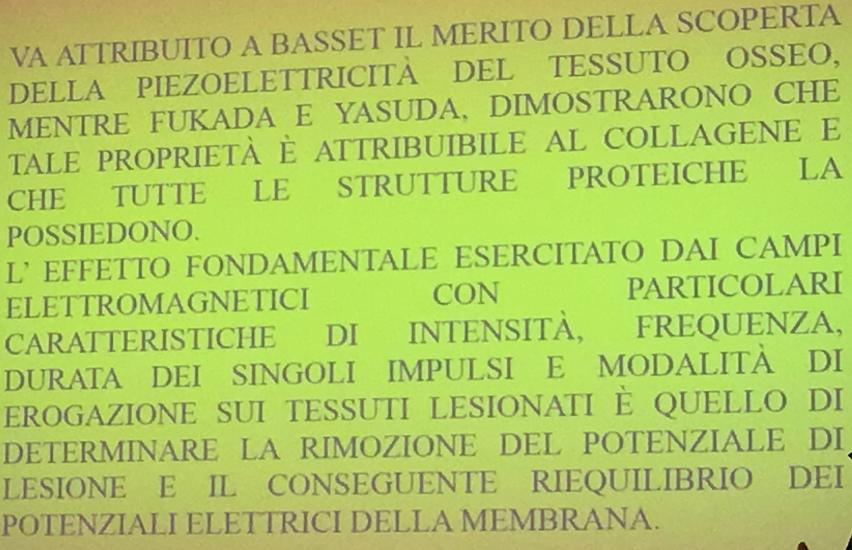
\includegraphics[width=0.4\textwidth]{026/image1.png}
\end{figure}

L'effetto
sul tessuto è legato all'effetto sulla cellula, la quale stimolata e
parte di un tessuto su cui si riflettono poi le modificazioni.

\textbf{\emph{L'effetto sugli organi è legato all'intensità e alla
frequenza del campo magnetico.}} L'intensita viene valutata in Gauss, la
frequenza in Hertz.

Si parla di \emph{\emph{eliminazione del potenziale di lesione e
ristabilizzazione del potenziale di membrana.}} E' un effetto importante
perché un adeguato potenziale di membrana permette uno scambio ottimale
tra interno e esterno della cellula, garantendo l'omeostasi cellulare e
di conseguenza tissutale. L'esito dovrebbe quindi portare a un miglior
funzionamento del tessuto. Se così fosse veramente, basterebbe avere
apparecchiature con questo effetto di normalizzazione del potenziale di
membrana per stare benissimo. Non è cosi, questo apparecchio esiste, si
chiama \emph{ionorisonanza ciclotronica}, e questo effetto
particolarmente complesso nella realtà si tramuta poi in effetto
paradosso per alcuni soggetti. Alla base vi è, in soggetti predisposti,
la normalizzazione del potenziale di membrana, che agisce su tessuti
sensibili come il tessuto nervoso e che può creare effetti collaterali
come insonnia, facile irritabilità, reazioni eccessive di sudorazione,
vomito. Di conseguenza questo tipo di trattamento e le apparecchiature
per l'applicazione sono state progressivamente abbandonate nel tempo.

\begin{figure}[!ht]
\centering
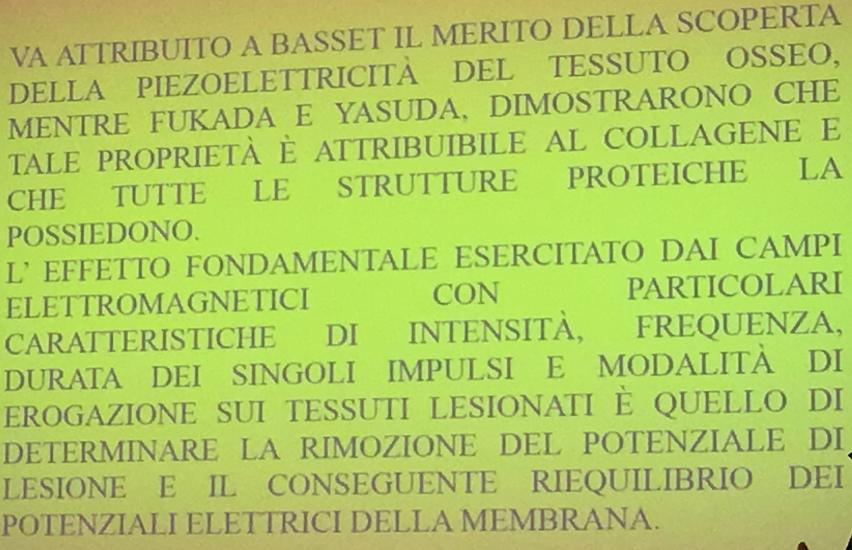
\includegraphics[width=0.4\textwidth]{026/image1.png}
\end{figure}

Gli
effetti più sfruttati in ambito terapeutico sono gli effetti meccanici,
soprattutto a livello del tessuto osseo. L'effetto meccanico sul tessuto
osseo è una stimolazione della deposizione di tessuto, quindi una
\emph{\emph{stimolazione degli osteoblasti}}. La maggiore applicazione è
in campo ortopedico nei ritardi di consolidazione delle fratture, perchè
tramite un'azione di compressione si ha una stimolazione
dell'osteogenesi. (poi nello specifico è stato visto che può cambiare
l'azione a seconda della posizione in cui va a stimolare perchè la
polarizzazione può essere positiva o negativa a seconda delle
circostanze).

\emph{E' stato sperimentalmente dimostrato che l'osso lungo sottoposto
ad azione deformante (es flessione, anche solo durante la deambulazione)
forma cariche + sulla superficie convessa, zona di trazione, cariche --
sulla superficie concava, di compressione (piezoelettricità ossea). Si è
visto che la zona negativa è la zona di deposizione ossea, la positiva
di riassorbimento.}

\emph{Si è dunque ipotizzato che le cariche negative potessero, in
qualche modo, favorire la deposizione ossea e si è notato che
l'applicazione di un catodo (catodo ha carica -) in sede di frattura
ossea (impiantando il catodo sull'osso) effettivamente favorisce la
deposizione di sostanza ossea e quindi la guarigione (parliamo degli
anni '70). Ovviamente l'applicazione diretta di un catodo a livello
dell'osso aveva numerose controindicazioni ( focolai di osteomielite,
più interventi chirurgici, rischio di infezioni..). Per ovviare a questo
problema, si è pensato di applicare un campo magnetico pulsante che,
variando d'intensità, producesse, per induzione, una corrente elettrica
che andasse ad agire sull'osso. Abbiamo quindi un duplice effetto:
quello magnetico e quello elettrico.}

\emph{È importante rispettare i tempi, i dosaggi d'applicazione e la
sede di applicazione per evitare le cause di insuccesso.}

\emph{A livello delle cellule dell'osso, ricerche sperimentali hanno
dimostrato che l'applicazione di questa metodica determina aumento
dell'attività metabolica cellulare e la maggior produzione di collagene,
influenza inoltre l'orientamento delle fibre di collagene e predispone
ad una loro più fitta deposizione. Parallelamente aumenta anche la quota
di minerali che possono depositarsi a livello di questo collagene. Oltre
a questo effetto metabolico-organizzativo, c'è anche una stimolazione
alla neoangiogenesi che permette il nutrimento del tessuto che si va
formando.}

\emph{Inoltre il segnale elettromagnetico sembrerebbe favorire la
riattivazione di cellule quiescenti come cellule mesenchimali del
periostio, monociti e fibroblasti che acquisterebbero attività
osteoblastica.}

Questo è un esempio di trattamento di una necrosi della testa femorale,
che può essere di origine vascolare, traumatica o di altra origine. Ci
sono due opzioni di trattamento:

\begin{itemize}
\item
  \textbf{conservativo}, per cercare di salvare la testa femorale
\item
  \textbf{chirurgico,} se fallisce quello conservativo, e che spesso
  viene usato in elezione.
\end{itemize}

Sono state fatte delle sperimentazioni per 6 ore giornaliere con
un'intensità di 20-30 Gauss e si è vista una risposta in diversi casi.
Si è visto quindi che questo trattamento ha anche un effetto di
\emph{biostimolazione}, perchè se si normalizza il potenziale di
membrana e si ha una biostimolazione che porta a una rigenerazione
tissutale.

Un altro campo d'azione è l'osteocondrosi, giovanile, o meglio
localizzata, perché quella giovanile è abbastanza ampia e può colpire la
colonna. Nel morbo di Osgood Schlatter, che è un osteocondrosi a livello
dell'apofisi tibiale, si frammenta il nucleo di ossificazione
dell'apofisi tibiale in soggetti giovani che fanno attività sportiva
precocemente. Spesso e volentieri questo viene identificato da diversi
medici come i ``famosi dolori da accrescimento'' che fanno male alle
ginocchia, quando non è cosi perché è una frammentazione del nucleo che,
sottoposto a sollecitazioni meccaniche, essendo fibroso, tende a
modificare il suo aspetto, a frammentarsi e poi a trasformarsi
successivamente con l'età. Raggiungendo la maturazione si crea una zona
di possibile sollecitazione meccanica dove può insorgere una tendinosi
del tendine rotuleo e una sintomatologia dolorosa. Stesso discorso vale
ad esempio per un'altra osteocondrosi che è quella calcaneale. Anche
questa si verifica precocemente per attività sportiva ed è abbastanza
frequente, soprattutto in sport come il calcio e altri sport di
resistenza. Anche nell'osteocondrosi si può usare un'applicazione con
frequenze di 50-100 Hz e intensità 60-400 Gauss.

Gli apparecchi presenti in commercio non raggiungono potenze cosi
elevate, viaggiano generalmente a 100-150-200 Gauss, potenze più alte si
hanno solo in pochi apparecchi. Anche i campi elettromagnetici pulsati
usati in terapia non hanno potenze cosi alte, ma sempre attorno ai 200
G. Esistono dei magneti naturali che possono raggiungere potenze anche 4
volte più alte.

I campi elettromagnetici sono utilizzati anche nelle arteriopatie e
nelle flebopatie.

Nella \textbf{patologia vascolare} si usano 4 ore giornaliere di
applicazione ad alta frequenza e bassa intensità portano a una buona
azione sull'edema post operatorio, su lesioni cutanee venose (ulcere),
con azione di biostimolazione. In questo caso con biostimolazione si
intende un effetto analgesico e di riparazione tissutale con riduzione
del tempo di cicatrizzazione. Se si vuole ottenere un effetto di
miglioramento sul circolo bisogna utilizzare basse intensità e frequenze
poco più alte, o meglio ancora basse intensità e basse frequenze. (NB:
L'alta frequenza serve per agire in profondità).

\subsection{Controindicazioni e precauzioni }

\begin{itemize}
\item
  Portatori di pacemaker
\item
  Gravidanza
\item
  Neoplasie
\item
  Stati emorragici/trombotici (tromboflebite, flebotrombosi, TVP)
\item
  Versamenti ematici, perché l'effetto termico va a vasodilatare la
  zona, aumentando la vascolarizzazione e l'afflusso di sangue
  peggiorando il versamento.
\end{itemize}

Gli \textbf{effetti collaterali}, che regrediscono al cessare
dell'applicazione, dipendono esclusivamente dal tempo di esposizione e
possono essere:

\begin{itemize}
\item
  Sonnolenza
\item
  Parestesie
\item
  Insonnia
\item
  Ipotensione
\item
  Irritabilità
\item
  Astenia
\item
  Cefalea
\end{itemize}

Sembra avere molte più controindicazioni che indicazioni, però viene
utilizzata e se usata in maniera adeguata è abbastanza efficace. In
commercio esisitono apparecchi abbastanza efficaci soprattutto quelli
che hanno un effetto di biostimolazione. Igea, un'azienda bolognese,
produce quattro tipi di apparecchi: uno di questi ha effetti di
stimolazione importanti sugli edemi post traumatici a livello osseo, e
questo rappresenta un dato importantissimo perchè un edema post
contusivo o post distrattivo osseo nell'articolazione sotto astragalica
possono essere gestiti in questo modo con risultati buoni tramite
applicazioni di 4 ore a frequenza definita di 50 Hz e intensità di 75 G.
Questo per dire che sono stati fatti studi importanti ed esistono altri
apparecchi per i ritardi di consolidazione.

\subsection{Usi in medicina }

Campi magnetici pulsati a bassa frequenza sono usati per i ritardi di
consolidazione.

Campi magnetici ad alta frequenza non vengono utilizzati in maniera
importante.

\section{Magneti naturali}

Esistono in natura sostanze come il \textbf{Borio}, il
\textbf{Berillio}, il \textbf{Neotinio} che hanno un grosso effetto
magnetico. Si usano su una base in modo che vi sia un orientamento del
campo magnetico in una sola polarità, affinché vi siano 4 poli che
confluiscono in un punto preciso in modo da aumentare la potenza di
questi magneti naturali. Possono raggiungere potenze anche di più di
1000G, con effetti straordinari su riparazione e tempi di riparazione
delle fratture.

\subsection{Frattura scafoide carpale composta}

\begin{figure}[!ht]
\centering
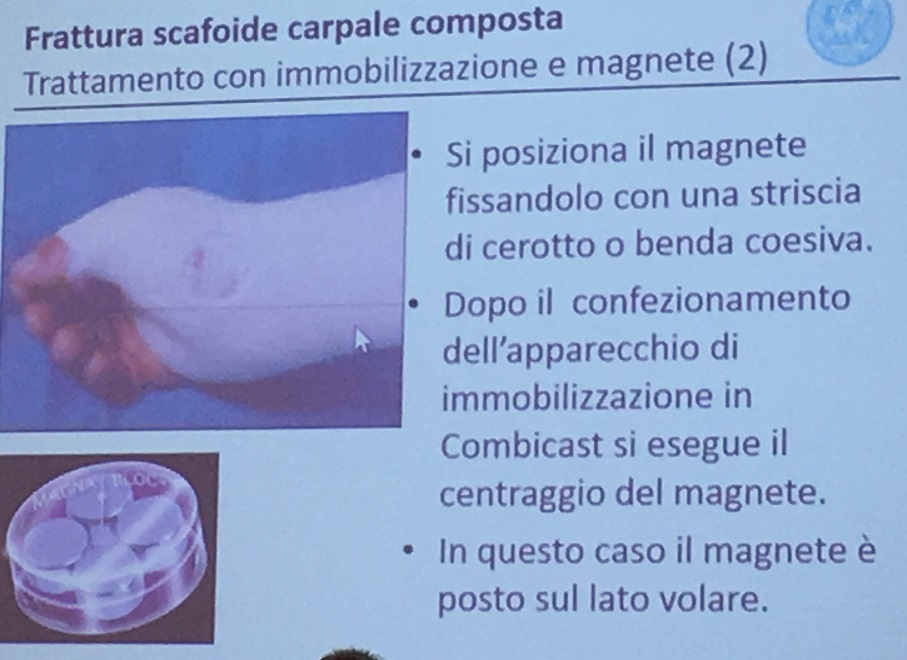
\includegraphics[width=0.4\textwidth]{026/image3.jpeg}
\end{figure}

\begin{figure}[!ht]
\centering
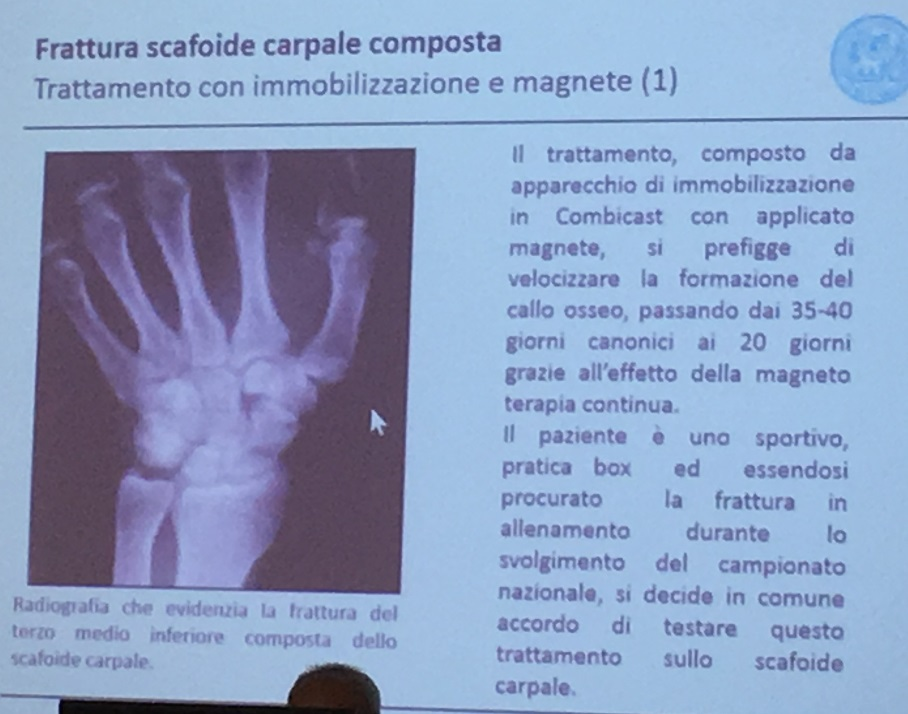
\includegraphics[width=0.4\textwidth]{026/image4.jpeg}
\end{figure}

Questo
paziente ha fatto un trattamento di 20 gg di magnetoterapia continua,
per velocizzare la formazione del callo osseo (35-40 gg normali). Il
magnete si applica e si fissa sotto guida radiografica in una
fenestratura creata nell'apparecchio gessato. Generalmente questi
magneti hanno 2 cm di diametro, 5 cm di altezza, 4 blocchi di neotinio
ferro-boro, 4 poli magnetici (2 positivi e 2 negativi). Si applicano in
modo da mettere il polo negativo a contatto con la zona da trattare. La
potenza può arrivare fino a 12500 G perché vi è la possibilità di
controllare la polarizzazione.

Questi magneti funzionano benissimo sullo scafoide e sulle fratture di
clavicola. L'effetto importante sullo scafoide è dovuto al fatto che sia
vascolarizzato, di conseguenza possono esplicare l'azione a livello dei
vasi migliorando l'afflusso tissutale e creando la possibilità di una
riparazione migliore, oltre al fatto che hanno un effetto di prevenzione
della necrosi locale. Questo tipo di trattamento non è automatico, molti
ortopedici non lo conoscono neanche, o addirittura lo ignorano. Da uno
studio è risultato che i tempi di riparazione siano accorciati in
maniera importante, con una riduzione media del 30\%. Bisogna pensare
anche al discorso dal punto di vista riabilitativo, perché se un
paziente resta immobilizzato per 40 giorni e invece si può ridurre
questo tempo a 25-30 giorni, significa togliere prima il gesso, togliere
prima il tutore, iniziare un trattamento riabilitativo precoce ed avere
maggiori possibilità di un recupero migliore. Inoltre, un altro
vantaggio di questi magneti è la facile applicazione. L'unico handicap è
che i magneti naturali venivano prodotti in America, da una sola ditta,
che non importa più in Italia. I cinesi hanno fatto dei magneti, però si
sono concentrati sulla forza di attrazione. Hanno prodotto magneti della
grandezza di un pisello e dell'altezza di 2 cm capaci di sollevare una
bicicletta. Però devono ancora capire che bisogna sfruttare l'effetto
paramagnetico e usare il discorso dei dipoli. Sono in atto studi cinesi
per produrre un magnete tripolare con una potenza di 20000 G. i magneti
naturali potrebbero essere il trattamento del futuro, permettendo di
applicare al posto del gesso un tutore con un magnete, risolvendo la
patologia precocemente e iniziando sempre precocemente il trattamento
riabilitativo.

L'indicazione base per la magnetoterapia è la patologia
ortopedica-traumatica, però anche sull'osteoporosi e nella
neuroartrodistrofia potrebbe avere dei buoni risultati. Per
l'osteoporosi è l'onda meccanica di compressione che dà l'effetto di
stimolazione, tanto è vero che adesso si usano apparecchi per vibrazione
locale. Nella neuroartrodistrofia vi è una disfunzione simpatica e un
piccolo effetto di biostimolazione a magnetoterapia bassa può essere
utile. La ionorisonanza ciclotronica lavora con frequenze di 1-5 Hz e
potenze di 1-2 G, dando effetti blandi ma efficaci. Questo sistema è
formato da un lettino formato da tante fasce unite tra loro (circa 12) e
ogni fascia ha dei sistemi con i campi magnetici.

\subsection{Modalità di applicazione dei campi magnetici normali}

L'apparecchiatura è costituita da un lettino con due solenoidi e il
campo magnetico è prodotto all'interno dei solenoidi. Se si posizione
tra i due solenoidi una calamita, questa vibra lo stesso. Per dire che
il campo magnetico non è prodotto solo all'interno ma anche al di fuori.
Questo è il motivo per cui i telefonini producono campi elettromagnetici
nocivi.

Esistono anche apparecchi portatili ma sono variabili. Quelli più
utilizzati in terapia sono i campi magnetici pulsatili.

La magnetoterapia rientrava tra le terapie che potevano essere erogate a
regime di convenzione solo entro certi limiti e in alcune patologie
specifiche. Dall'anno scorso non è proprio più in convenzione e non
rientra nei livelli essenziali di assistenza (LEA).

I campi magnetici sono utilizzati negli accelerometri, i quali sono
presenti anche in tutti i telefonini. Tanto è vero che hanno prodotto
delle microcalamite che vanno applicate dietro agli apparecchi che
producono elettromagnetismo per assorbire ed evitare che
l'elettromagnetismo si diffonda nell'ambiente. Ci sono alcune aziende
che hanno prodotto microcalamite da applicare ai cellulari e pare che
funzionino.

\emph{Domanda: maggiore è la potenza in Gauss maggiore è l'effetto
benefico? Ci sono dei limiti? }

Risposta: non è cosi lampante questa correlazione e non è ancora stata
indagata in maniera certa. Vi sono applicazioni diverse: alta frequenza
bassa intensità o campi elettromagnetici pulsatili, in cui il campo
elettromagnetico parte da un livello fino a raggiungere un massimo e
ritorna a scendere, poi dopo una pausa riparte. L'effetto non deve
essere continuo ma alternato, pulsato, e anche i campi elettromagnetici
pulsati di solito non hanno delle potenze alte, raggiungono i 100G, per
quanto riguarda il trattamento a domicilio. L'applicazione in
ambulatorio medico dura mezz'ora, un'ora massimo, quelli a domicilio
hanno applicazioni medie di 4 ore, perché l'interruzione è data dal
programma.

\emph{Domanda: Il vantaggio dei magneti naturali di fornire potenze
elevatissime allora dove sta? }

Risposta: il vantaggio è un aspetto che deve essere ancora evidenziato
con alcuni studi più accurati. Sono magneti naturali e di conseguenza
dovrebbero fare qualcosa di diverso rispetto a un campo magnetico
prodotto da un campo elettrico. La differenza potrebbe essere un effetto
biologico diverso magari sulla membrana cellulare e di conseguenza avere
l'effetto non tanto legato alla potenza ma forse al fatto che magari
agiscono in maniera diversa sulle membrana. In teoria più è alta la
potenza più è l'effetto meccanico.

\emph{Domanda: Per l'osteomielite è un trattamento possibile?}

Risposta: l'osteomielite è un problema grosso e complesso. Utilizzare un
campo magnetico potrebbe significare di fare in modo che l'infezione
abbia la capacità di espandersi maggiormente, perchè si va a lavorare
sul circolo che rappresenta un modo per disseminare l'osteomielite.
Nelle infezioni dare calore, vasodilatare o agire sul circolo è
deleterio, sempre.

\begin{figure}[!ht]
\centering
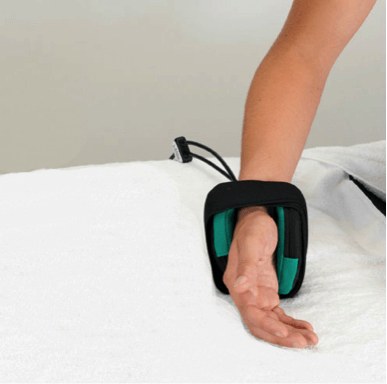
\includegraphics[width=0.4\textwidth]{026/image5.png}
\end{figure}

\begin{figure}[!ht]
\centering
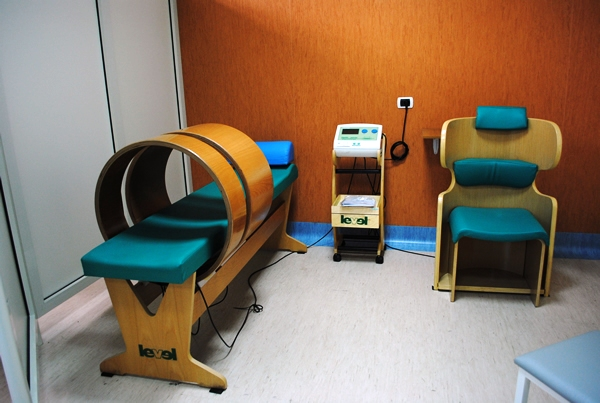
\includegraphics[width=0.4\textwidth]{026/image6.jpeg}
\end{figure}

\begin{figure}[!ht]
\centering
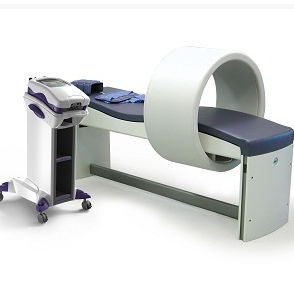
\includegraphics[width=0.4\textwidth]{026/image7.jpeg}
\end{figure}
